\section{Мета практикуму}
Практично ознайомитися із алгоримом дискретного логарифмування Сільвера-Поліга-Геллмана, реалізувати зазначений метод. Практично оцінити складність роботи алгоритму.

\subsection{Постановка задачі та варіант}
\begin{tabularx}{\textwidth}{X|l}
\textbf{Треба реалізувати} & \textbf{Зроблено} \\
\hline
Алгоритм Сільвера-Поліга-Геллмана & Алгоритм Сільвера-Поліга-Геллмана \checkmark\\
\end{tabularx}

\section{Хід роботи/Опис труднощів}
На початку реалізації практикуму трохи виникли незначні проблеми із розумінням того, як треба зберігати степені для обчислення $x_{i}$ (от саме пункти 3., 4. у самому алгоритмі), але все обійшлося, як тільки почав їх реалізовувати. :) 

\begin{figure}[h]
			\center{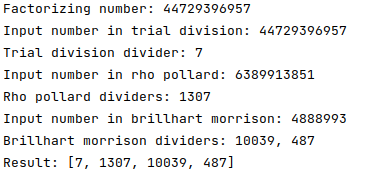
\includegraphics[scale = 0.45]{example1}}
			\caption{Пункти 3., 4. у алгортимі}
			\label{fig:image}
		\end{figure}

Основна проблема у мене виникла із тим, як треба розв'язувати рівняння. Так, треба було застосувати \textit{Китайську Теорему про Лишки}, але від початку неправильно реалізував обрахунок $M_{i}$ елементів, тому шукав, чому при обчисленні оберненого елементу на вхід приходить число $0$, адже для 0 не існує його.

Також були труднощі не стільки у самому алгоритмі, а скільки у його реалізації із типами чисел у алгоритмах факторизації. Саме там, ще не знав про реалізацію великих чисел, тому там усі числа упираються у тип $u128$ (тип, що містить беззнакові числа довжини 128 біт). Тому, у цьому практикумі прийшлося підлаштовуватися під цей недолік.

Але, не зважаючи на деякі проблеми, на мою думку, цей алгоритм дискретного логарифмування виявився набагато легшим, ніж Брілхарта Морісона у попередньому практикумі.
Навчений попереднім досвідом, одразу використовував бібліотеку великих чисел у rust --- \href{https://crates.io/crates/num-bigint}{\textit{\underline{num-bigint}}}.

\pagebreak

\section{Результати дослідження}
У результаті маємо, що:
\begin{enumerate}
\item Алгоритм Сільвера-Поліга-Геллмана --- дуже ефективниий для вирішення $dlp$, саме для чисел, які розкладаються на багато малих дільників, доприкладу: 


\begin{figure}[h]
			\center{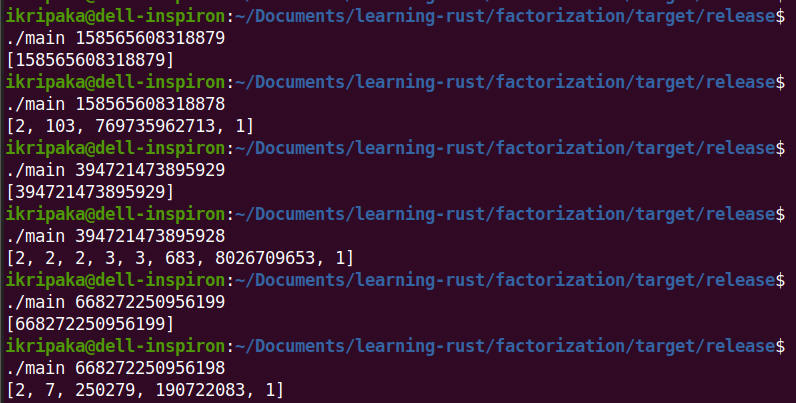
\includegraphics[scale = 0.4]{bad_numbers_example1}}
			\caption{Приклад поганих чисел для Сільвера-Поліга-Геллмана}
			\label{fig:image}
		\end{figure}
		
\begin{figure}[h]
			\center{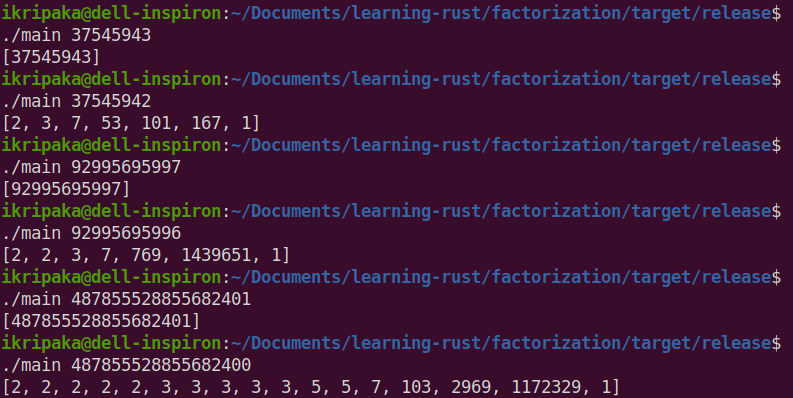
\includegraphics[scale = 0.4]{good_numbers_example1}}
			\caption{Приклад добрих чисел для Сільвера-Поліга-Геллмана}
			\label{fig:image}
		\end{figure}

\item Проблема полягає у тому, що для формування таблички передобчислених значень треба перебрати числа, до прикладу, для $6682722509956199 = 2*7*250279*190722083$ --- максимальна кількість ітерацій буде $190722083$, що для однопоточної програми може викликати часові проблеми. На мою думку, це можна вирішити за допомогою розпаралелювання перебору цих усіх значень.

\end{enumerate}

\pagebreak
\section{Продуктивність}
\vspace{3mm}
Після обрахунків вийшло наступне:

{\def\arraystretch{2}
\begin{tabularx}{\textwidth}{||r|c|l||}
\renewcommand{\arraystretch}{1.7}
  \textbf{Числа(a, b, n)} & \textbf{dlp алгоритм} &  \textbf{Розклад числа $(n-1)$} \\
\substack{(44,\\ 1229,\\ 6277)} & 391ns & [2, 2, 3, 523]\\
\substack{(70425,\\ 4498,\\ 98929)} & 82.973186ms & [2, 2, 2, 2, 3, 3, 3, 229]\\
\substack{(79791,\\ 7727,\\ 106621)} & 264.272183ms & [2, 2, 3, 5, 1777]\\
\substack{(5347363,\\ 1393557,\\ 5794511)} & 76.10528318s & [2, 5, 579451]\\
\substack{(32012782,\\ 4740726,\\ 37545943)} & 250.110651ms & [2, 3, 7, 53, 101, 167]\\
\substack{(431663093,\\ 527715071,\\ 633337597)} & 16.348184705s & [2, 2, 3, 3, 3, 47, 124771]\\
\substack{(5710238076,\\ 5213445017,\\ 6390644171)} & 250.787527ms & [2, 5, 41, 79, 1033, 191]\\
\substack{(62169854910,\\ 86077798599,\\ 92995695997)} & 185.391740656s & [2, 2, 3, 7, 769, 1439651]\\
\substack{(71428636448,\\ 180199541342,\\ 584842224173)} & \geqslant 13min & [2, 2, 41, 3566111123]\\
\substack{(4313558325450,\\ 6380632412530,\\ 9577259708671)} & \geqslant 11min & [2, 3, 3, 5, 31, 401, 8560373]\\
\substack{(13637999129366,\\ 2111433979175,\\ 15710549366693)} & \geqslant 20min & [2, 2, 3670967, 1069919]\\
\substack{(187165199375552,\\ 22166621073359,\\ 336305574949727)} &  \geqslant 4min & [2, 383, 193, 7717, 294781]\\
\substack{(2629622656603408,\\ 3806920734785279,\\ 3821293645373207)} & 69.077615454s & [2, 36493, 127711, 409961]\\
\substack{(31359535267603010,\\ 3969189589541717,\\ 91983358119398483)} & 404.263866988s & [2, 11, 59, 4637, 4547, 3361031]\\
\substack{
(107477375094958706,\\ 438527732551443546,\\ 487855528855682401)} & 139.449256575s & [2, 2, 2, 2, 2, 3, 3, 3, 3, 3, 5, 5, 7, 103, 2969, 1172329]\\

\end{tabularx}}

\vspace{5mm}
\textbf{Оцінка продуктивності}:
\begin{enumerate}
\item Моя реалізація алгоритму має обмеження на вхід чисел $<340282366920938463463374607431768211455$ (39 значні числа).
\item Практично межа проходить на 18, 19, ... значних числах, адже там уже іде розклад на числа $>1000000$, що уже важко перебрати.
\end{enumerate} 

\section{Висновки}
За допомогою практикуму "Застосування алгоритму дискретного логарифмування" дізнався як вирішуються dlp задачі на вище зазначеному алгоритмі.

У результаті одержав, що Сільвер-Поліг-Геллман повинен використовуватися у парі із іншим алгоритмом, до прикладу, із BabyStep-GiantStep, або із Pollard's Kangaroo Algorithm, який активно модифікується за домогою додавання різної кількості "wild kangaroo", "tame kangaroo", та інших модифікацій різних відомих алгоритмів для вирішення дискретного логарифма, або спробувати реалізувати розпаралелювання передобчислень, які займають більшу кількість роботи алгоритму. 

	




